En geometría computacional, necesitaremos una forma de representar a los objetos geométricos en código, a los puntos del plano los representaremos como un par de coordenadas de $(x,y)$ con las operaciones usuales aplicadas coordenada a coordenada. 

\lstinputlisting[language=C++]{./tex/geo/codes/punto.cpp}
Como definimos nuestra propia estructura es necesario que también definamos los comparadores para poder decidir si dos puntos son iguales o no.
\lstinputlisting[language=C++]{./tex/geo/codes/comparator.cpp}
Nótese que el definir un comparador para decidir si un punto es ''menor'' a otro, no es tan fácil qué hacer por lo que usualmente dependiendo el caso los ordenaremos, frecuentemente nos convendrá ordenarlos de forma horaria o antihoraria de acuerdo a los vectores que corresponden los puntos, la pregunta ahora consiste en ¿cómo hacer esto?, antes de ver una técnica para hacerlo, recordaremos algunas operaciones que podemos hacer entre puntos.
\\\\En primer lugar tenemos el producto punto, dados dos puntos este nos ayuda a medir qué tanto dos vectores apuntan a la misma dirección, si el producto punto es positivo, los vectores apuntan a direcciones similares, si es cero, los vectores son perpendiculares y si es negativo, entonces los vectores apuntan en direcciones opuestas, en programación competitiva este se calcula simplemente con las coordenadas.
\lstinputlisting[language=C++]{./tex/geo/codes/dot.cpp}
Nótese que por como lo calculamos si hacemos el producto punto de un vector consigo mismo tendremos la norma de este al cuadrado.
\\\\Otro concepto que nos será relevante recordar es el producto cruz entre dos vectores (denotado $a \times b$), este nos dará el área orientada del paralelogramo que forman dos vectores, con orientada nos referimos a que si calculamos $a \times b$ será el área del paralelogramo negativa, en cambio $b \times a$ nos la dará positiva, esto nos da una noción de si un vector está a la ''izquierda'' o ''derecha'' de otro.
\begin{center}
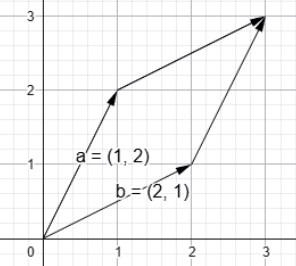
\includegraphics[scale=.5]{./tex/geo/pics/cross1.png}
\end{center}
la implementación también es sencilla y nos da una forma rápida de comprobar si tres puntos son colineales.
\lstinputlisting[language=C++]{./tex/geo/codes/cross.cpp}
Con lo anterior ya tenemos las herramientas suficientes para resolver nuestro problema de ordenar los puntos del plano de forma horaria o antihoraria alrededor de un punto.
\\
Supongamos que queremos ordenar los puntos del plano de forma antihoraria respecto al origen y con una referencia de ''inicio'' que tomaremos como $v=(0,1)$.
\\Notemos que si tenemos un conjunto de puntos $A$, podemos dividir el plano en dos partes, la primera que llamaremos $N$ que tendrá a todos los puntos que estén a la izquierda de $v$ y todos los puntos que sean colineales apuntando a la misma dirección, la segunda se llamará $S$ y serán los restantes, es decir, aquellos a la derecha de $v$ y los colineales que apuntan en dirección opuesta es decir, los puntos en el área roja estarían en $N$ y los del área azul en $S$.
\begin{center}
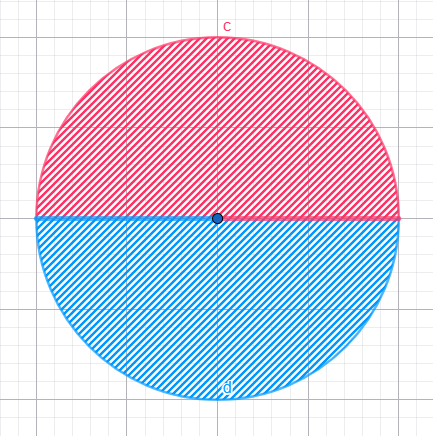
\includegraphics[scale=.5]{./tex/geo/pics/sort.png}
\end{center}
Entonces de aquí que digamos que para un punto $x$ en $A$, $x$ está en $N$ si y sólo si se cumple que $v\times x >0$ o $v\cdot x >0$ y además $v\times x=0$, estás siendo las operaciones de producto punto y cruz que vimos arriba, con esto podemos hacer una función que nos verifique si un punto de $A$ está o no en $N$ facilmente
\lstinputlisting[language=C++]{./tex/geo/codes/sort1.cpp}
Una vez dividido en dos partes notemos que dados $x$ y $y$, podemos decir que $x < y$ si $x \in N$ y $y \in S$ o ambos están en la misma parte y además $x \times y >0$, para esto entonces sólo nos basta definir un operador como sigue que es más fácil de manipular.
\lstinputlisting[language=C++]{./tex/geo/codes/sort2.cpp}

